\documentclass[lecture_notes.tex]{subfiles}

\begin{document}

\notestitle{Session 5}{Matrix Product States for Fermionic Models}%
  {mps\_many\_body\_fermionic.ipynb}{Sessions 3--4 (exact diagonalization directly in the fermionic
  basis; matrix product states for spin chains)}

\section*{Contents and goals}
Let us recall where we left things. In Session 3 we redid our many-body program directly in the
fermionic basis, with no product-state restriction at all, and it worked beautifully: we recovered
the exact spinless charge-density-wave transition and genuine spin-charge separation in the Hubbard
model. But we hit exactly the same wall we always hit with exact diagonalization, the Hilbert space
grows as $4^L$, and we were stuck around $L\sim 12$--$16$ sites. In Session 4 we built the fix,
matrix product states, but we only ever applied it to \emph{spin} Hamiltonians. Today we close the
loop: we are going to solve interacting \emph{fermionic} Hamiltonians with tensor networks, at
system sizes of a hundred sites or more, by first mapping them onto spin Hamiltonians through the
Jordan-Wigner transformation and then reusing every piece of MPS machinery we already built. Along
the way we will redo the Session 3 spinless and Hubbard results at a scale where the physics is
unambiguous, meet two genuinely new diagnostics, pairing correlators and the correlation entropy,
and finish, since this is the last session of the course, with the general tensor-network algorithm
that has been quietly running underneath everything since Session 4.

\section*{Learning outcomes}
By the end of this session, you should be able to:
\begin{itemize}[nosep]
  \item Map a fermionic Hamiltonian onto an equivalent spin Hamiltonian via the Jordan-Wigner
    transformation, and explain why nearest-neighbor hopping needs no explicit string.
  \item Use MPS at system sizes of $\sim100$ sites to locate a genuine quantum phase transition
    that exact diagonalization could not resolve sharply.
  \item Compute pairing correlators, including their enhancement toward Cooper-pair-like behavior
    under attractive interactions, and use the correlation entropy to judge how far a ground state
    is from a mean-field, single-Slater-determinant description.
  \item Describe, at a diagrammatic level, how the DMRG sweep optimizes an MPS tensor by tensor,
    and place MPS/DMRG within the broader family of tensor-network methods (PEPS, MERA).
\end{itemize}

\section{From spins to fermions: the Jordan-Wigner mapping}
\label{sec:jw}
The question we want to answer first is almost philosophical: are spin models and fermionic models
secretly the same thing? On the face of it they look like different kinds of objects. A fermionic
Hamiltonian is built from operators $\cre{i},\ann{i}$ that anticommute on different sites,
$\{\ann{i},\cre{j}\}=\delta_{ij}$, while a spin-$\tfrac12$ Hamiltonian is built from operators
$S_i^x,S_i^y,S_i^z$ that \emph{commute} on different sites and only satisfy a nontrivial algebra
on the same site. Tensor networks, as we built them in Session 4, are fundamentally bosonic
objects: an MPS is just a product of matrices, one per site, and nothing in that construction knows
about fermionic minus signs. So if we want to use MPS to solve fermionic Hamiltonians, and that is
exactly what we want to do today, we first need a dictionary that turns a fermionic Hamiltonian into
an equivalent spin Hamiltonian.

\subsection{Matching the local Hilbert spaces}
The first step is easy. A single fermionic site has exactly two states, empty $\ket{0}$ and
occupied $\ket{1}=\cre{}\ket{0}$, because $\cre{}\cre{}=0$ forbids double occupancy. A single
spin-$\tfrac12$ also has exactly two states, $\ket{\dn}$ and $\ket{\up}$. So let us just identify
them site by site,
\begin{equation}
  \ket{0} \leftrightarrow \ket{\dn}, \qquad \ket{1} \leftrightarrow \ket{\up},
\end{equation}
and correspondingly identify the operators that move between them: $\cre{}$ takes empty to occupied,
exactly like $S^+$ takes down to up, so we would like to say $\cre{}\leftrightarrow S^+$,
$\ann{}\leftrightarrow S^-$, and, since $n=\cre{}\ann{}$ is $0$ or $1$ while $S^z$ is $\mp\tfrac12$,
\begin{equation}
  S_i^z = n_i - \tfrac12.
\end{equation}
So far this looks like a clean bijection between the two Hilbert spaces. But notice the sentence we
just glossed over: fermionic operators on different sites \emph{anticommute}, while spin operators
on different sites \emph{commute}. That mismatch is not a technicality, it means the naive
identification $S_i^+\stackrel{?}{=}\cre{i}$ cannot possibly be right as it stands.

\begin{figure}[H]
  \centering
  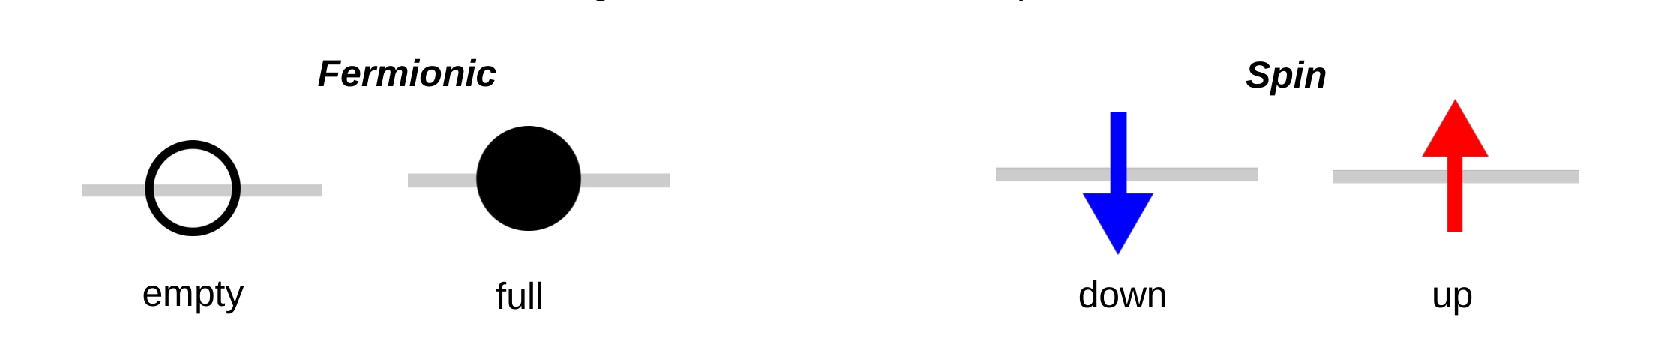
\includegraphics[width=0.80\textwidth]{figures/mps_fermionic/jw_hilbert_space.pdf}
  \caption{The local Hilbert spaces matched at the start of the Jordan-Wigner construction. A
    spinless fermionic site is either empty or occupied, and a spin-$\tfrac12$ site points either
    down or up, so the identification $\ket{0}\leftrightarrow\ket{\dn}$,
    $\ket{1}\leftrightarrow\ket{\up}$ is a clean bijection site by site. What the picture cannot
    show is the mismatch the rest of this section exists to repair: operators on different
    fermionic sites anticommute, while spin operators on different sites commute.}
  \label{fig:jw-local}
\end{figure}

\subsection{The string operator}
Let us see the mismatch explicitly, since it is the whole reason this section exists. Take the naive
guess $\widetilde S_i^+ \equiv \cre{i}$, $\widetilde S_j^- \equiv \ann{j}$ for $i\ne j$. Then
\begin{equation}
  \widetilde S_i^+ \widetilde S_j^- = \cre{i}\ann{j}, \qquad
  \widetilde S_j^- \widetilde S_i^+ = \ann{j}\cre{i} = -\cre{i}\ann{j},
\end{equation}
where the last step is just the fermionic anticommutation relation for $i\ne j$. So the naive guess
gives us two operators that \emph{anticommute}, $\widetilde S_i^+\widetilde S_j^- =
-\widetilde S_j^-\widetilde S_i^+$, whereas genuine spin operators on different sites, being
independent two-level systems glued together with an ordinary tensor product, absolutely must
\emph{commute}, $S_i^+S_j^- = S_j^-S_i^+$. This is precisely the anticommutation-versus-commutation
mismatch we flagged above, and it means we need to dress the naive guess with something that fixes
the sign.

The fix is the \textbf{Jordan-Wigner string}. Order the sites along the chain, and define, for every
site $i$, the operator
\begin{equation}
  K_i \equiv \prod_{j<i}\left(1-2n_j\right),
\end{equation}
the parity of the number of fermions sitting to the left of site $i$: $K_i=+1$ if an even number of
sites to the left are occupied, $K_i=-1$ if odd. Since $K_i$ is built entirely out of number
operators $n_j=\cre{j}\ann{j}$, which are quadratic in fermionic operators, $K_i$ itself commutes
with any fermionic operator on a different site (two sign flips cancel), even though it looks like a
long, complicated string of anticommuting objects. It is also Hermitian and unitary, $K_i^2=1$. With
this in hand, the correct dictionary is
\begin{equation}
  S_i^+ = \cre{i}K_i, \qquad S_i^- = \ann{i}K_i, \qquad S_i^z = n_i - \tfrac12.
  \label{eq:jw}
\end{equation}
One can check, by direct computation using $K_i^2=1$ and the fact that $K_i$ commutes with operators
on other sites, that Eq.~\eqref{eq:jw} reproduces exactly the correct spin algebra: $[S_i^\alpha,
S_j^\beta]=0$ for $i\ne j$, and the usual $\mathfrak{su}(2)$ algebra on the same site. The string is
not optional decoration, it is the one piece of bookkeeping that makes a fermionic Hilbert space and
a spin Hilbert space, which are literally the same vector space, carry consistent operator algebras.

\subsection{Why nearest-neighbor hopping barely notices the string}
\label{sec:nnhop}
The reason this mapping is actually useful in practice, rather than just a mathematical curiosity,
is a small miracle that happens for nearest-neighbor terms. Take $i<j$ and work out the general
spin bilinear $S_i^+S_j^-$ in terms of fermions. Writing $K_j = K_i(1-2n_i)\prod_{i<k<j}(1-2n_k)$
and using $K_i^2=1$ together with the operator identity $\cre{i}(1-2n_i)=\cre{i}$ (creating a
particle on an already-doubly-forbidden site trivially just annihilates the extra term, since
$\cre{i}n_i=0$), a short calculation gives
\begin{equation}
  S_i^+S_j^- = \cre{i}\ann{j}\prod_{i<k<j}\left(1-2n_k\right), \qquad i<j.
  \label{eq:jwstring}
\end{equation}
So in general, hopping an electron from $j$ to $i$ really does require dragging a whole string of
$S^z$ operators across every intervening site. But look at what happens for the special case
$j=i+1$: the product in Eq.~\eqref{eq:jwstring} runs over an empty range and is simply $1$, so
\begin{equation}
  S_i^+S_{i+1}^- = \cre{i}\ann{i+1}.
\end{equation}
The string cancels completely. One can verify directly, using the same identities, that
$S_{i+1}^-S_i^+$ gives the very same operator, confirming that these two spin operators genuinely
commute as they must. So \emph{nearest-neighbor} hopping maps onto a completely local, string-free
spin term, while longer-range hopping does not. This is exactly why the Jordan-Wigner trick is such
a good match for one-dimensional, nearest-neighbor tensor-network methods: the models we actually
build MPS Hamiltonians for never need the string explicitly, it is only lurking in the background,
guaranteeing consistency, but never entering the actual Hamiltonian we hand to the solver.

\begin{figure}[H]
  \centering
  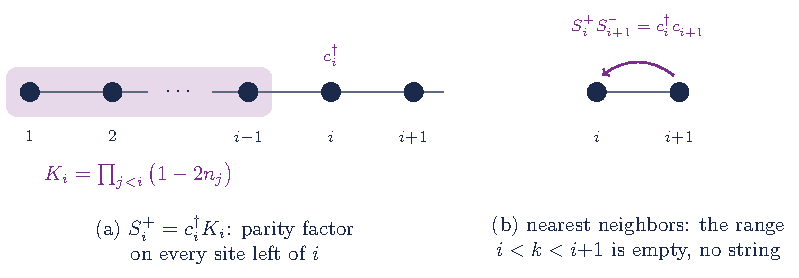
\includegraphics[width=0.90\textwidth]{figures/jw_string.pdf}
  \caption{The Jordan-Wigner string, and why it usually vanishes from sight. (a) The dictionary of
    Eq.~\eqref{eq:jw} attaches to $\cre{i}$ the parity factor $K_i=\prod_{j<i}(1-2n_j)$, one factor
    for every site to the left of $i$, shaded here. That trailing string is what repairs the
    mismatch between anticommuting fermions and commuting spins. (b) On a nearest-neighbor bond the
    product in Eq.~\eqref{eq:jwstring} runs over the empty range $i<k<i+1$, so the string collapses
    to $1$ and the spin bilinear reduces to the bare hopping. This is why the models we build
    matrix product state Hamiltonians for never meet the string explicitly.}
  \label{fig:jw-string}
\end{figure}

\subsection{The practical recipe}
Putting this together, the scheme we use for the rest of this session is: (1) start from an
interacting fermionic Hamiltonian; (2) rewrite it, site by site and bond by bond, as an equivalent
spin Hamiltonian using Eq.~\eqref{eq:jw}, which for nearest-neighbor models involves no explicit
strings at all; (3) solve this \emph{artificial}, unphysical-looking spin Hamiltonian with the MPS
machinery from Session 4; (4) map expectation values back to the fermionic language using the same
dictionary in reverse. From a practical standpoint, once this is set up, we can simply think of it
as a many-body solver for interacting fermions, and never worry about the string again, exactly the
way \texttt{dmrgpy}'s \texttt{fermionchain} class handles it internally for every calculation in
this notebook, which uses open boundary conditions throughout (Section~\ref{sec:jw}'s string
cancellation for nearest-neighbor hopping relies on a fixed left-to-right site ordering; on a
periodic chain the bond that closes the ring is not nearest-neighbor in that ordering and does pick
up an explicit, filling-dependent string, which is one more reason to stick to open chains).

For a Hubbard-type model with spin, each site carries two fermionic flavors, $\cre{i\up}$ and
$\cre{i\dn}$, so the recipe above needs one more choice: an explicit ordering of all $2L$ orbitals
along a single one-dimensional string before Eq.~\eqref{eq:jw} can be applied. The natural option is
to interleave them site by site, $\up_1,\dn_1,\up_2,\dn_2,\ldots$, so that same-site operators stay
adjacent; the alternative is to order all up-spins first and all down-spins after,
$\up_1,\ldots,\up_L,\dn_1,\ldots,\dn_L$, which keeps each spin sector's own hopping local but pushes
the on-site $U$ term into a long string. Either ordering is exact, and \texttt{dmrgpy} picks one for
us internally, but it is worth knowing this choice exists the next time you see a spinful
Jordan-Wigner string written down elsewhere.

\section{Large-scale replay: the spinless interacting chain}
\label{sec:spinless}
Let us put the machinery to work on a model we already know intimately from Session 3: spinless
fermions with nearest-neighbor hopping and nearest-neighbor repulsion,
\begin{equation}
  \Ham_{\mathrm{CDW}} = -t\sum_i\left(\cre{i}\ann{i+1}+\mathrm{h.c.}\right) + V\sum_i n_in_{i+1}.
  \label{eq:cdw}
\end{equation}
We already know its two extreme limits by heart: at $V=0$ it is a free-fermion metal, and as
$V\to\infty$ it becomes a charge density wave, one electron on every other site. What exact
diagonalization could never tell us cleanly, because $L\lesssim 16$ is simply too small to see a
sharp thermodynamic phase transition, is exactly where between these two limits the transition
happens, and MPS is going to answer that question for us.

\subsection{A pleasant surprise: this is the XXZ chain}
Before diving into the numerics it is worth pausing on the Jordan-Wigner image of
Eq.~\eqref{eq:cdw}, because it reconnects us to a model from Session 2. Using
Eq.~\eqref{eq:jw} and \eqref{eq:jwstring} for adjacent sites, the hopping term becomes
$-t(S_i^+S_{i+1}^-+\mathrm{h.c.}) = -2t(S_i^xS_{i+1}^x+S_i^yS_{i+1}^y)$, while the density term is
diagonal and trivial to translate, $n_in_{i+1} = S_i^zS_{i+1}^z + \tfrac12(S_i^z+S_{i+1}^z) +
\tfrac14$. Summed over the whole chain, the linear term $\tfrac12\sum_i(S_i^z+S_{i+1}^z)$ is, up to
the two uncancelled boundary sites, just $VS_{\mathrm{tot}}^z$, a uniform field that commutes with
the bulk hopping and simply shifts the energy at fixed filling (fixed $S_{\mathrm{tot}}^z$); the
$O(1)$ residual boundary field on the first and last site does not commute with the bulk hopping,
but it is a boundary effect that does not affect the bulk transition, so we drop it here, leaving
\begin{equation}
  \Ham_{\mathrm{CDW}} \;\longleftrightarrow\;
  \sum_i\left[-2t\left(S_i^xS_{i+1}^x+S_i^yS_{i+1}^y\right) + V S_i^zS_{i+1}^z\right] + \mathrm{const.}
  \label{eq:xxzferm}
\end{equation}
This is exactly the \textbf{XXZ chain} with anisotropy $\Delta \equiv V/(2t)$. Its exact
Bethe-ansatz solution places the transition between a gapless, easy-plane phase and a gapped,
N\'eel-ordered phase precisely at the isotropic Heisenberg point $\Delta=1$, i.e.\ at $V=2t$. Keep
that number in mind, we are about to rediscover it numerically.

\subsection{Charge order from a pinning field}
Because a translationally invariant Hamiltonian cannot spontaneously break translational symmetry
in a finite calculation (the ground state stays a symmetric superposition of the two CDW patterns),
the trick we use, both here and back in Session 1's mean-field discussion, is to add an
infinitesimal symmetry-breaking seed and see whether the bulk amplifies it or screens it out. Take a
chain of $L=100$ sites, add a tiny pinning term that favors slightly less charge on the first site
and slightly more on the last, and look at the resulting charge profile $\expval{n_i}$.

For strong interaction, $V=40t$, the pinning is all it takes: the whole chain locks into the
charge-ordered pattern, alternating high and low density from edge to edge. This tells us
unambiguously that we are inside the symmetry-broken phase. For moderate interaction, $V=t$, the
story is completely different: the charge does oscillate near the pinned edge, but the amplitude of
the oscillation decays as you move into the bulk, and by the middle of the chain the density has
relaxed back to the uniform value $\expval{n_i}=\tfrac12$. The bulk, in other words, actively wants
to screen out the perturbation, which is exactly the signature of a phase that does \emph{not} break
translational symmetry, even though $V=t$ is a sizeable interaction by any measure.

\begin{notebook}
Section ``Charge expectation value for weak and strong interactions.'' Plot $\expval{n_i}$ across
the $L=100$ chain for $V=40t$ and $V=t$ and confirm the two behaviors described above: saturated
order versus a decaying edge oscillation. Section ``Charge density in the presence of an impurity''
lets you repeat essentially the same diagnostic with the perturbation placed inside the chain
instead of at the edge, and moving it to the middle is a good way to convince yourself the effect is
a genuine bulk property and not an artifact of the boundary.
\end{notebook}

\subsection{The phase transition at $V_c$}
We can turn the qualitative picture above into a quantitative one by sweeping $V$ continuously and
tracking the bulk charge imbalance (or, equivalently, the site density deep in the chain, away from
the pinning) as a function of $V$. Below a critical value the bulk density stays flat at
$\expval{n}=\tfrac12$ no matter how hard we pin the edges; above it, the bulk itself develops a
finite charge imbalance, and the pinning field is only needed to select which of the two equivalent
sublattices orders. Numerically this happens at $V_c\approx 2t$, in beautiful agreement with the
exact XXZ result we derived in Eq.~\eqref{eq:xxzferm}. This is a genuine, thermodynamic-limit quantum
phase transition, a nonanalyticity in the ground state as a function of $V$ at zero temperature, and
it is one that a $L\sim 12$ exact-diagonalization calculation from Session 3 simply could not resolve
sharply: only at the $L\sim100$ scale that MPS gives us for free does the transition become crisp.

\begin{notebook}
Section ``Phase transition in a repulsive fermionic model.'' Sweep $V$ and locate where the bulk
density departs from $0.5$; check that this matches $V_c\approx2t$. Then repeat the whole
calculation with a much smaller chain, $L=10$, and see how much blurrier the transition becomes,
this is a direct, hands-on illustration of why we needed to leave exact diagonalization behind.
\end{notebook}

\section{Correlators as a diagnostic of the phases}
\label{sec:correlators}
Pinning fields and density profiles are intuitive, but they rely on us adding an explicit symmetry
breaking term. A cleaner, field-free diagnostic comes from nonlocal correlation functions, and it
generalizes something we already used for the Heisenberg model in Session 2.

\subsection{The nonlocal particle-particle correlator}
Define the single-particle correlator between the first site and site $n$,
\begin{equation}
  C(n) \equiv \expval{\cre{1}\ann{n}}.
\end{equation}
Physically this is exactly what a Kubo-formula response calculation would give you if you pinned
site $1$ infinitesimally and measured the induced amplitude at site $n$, so it packages the same
physics as Section~\ref{sec:spinless}'s pinning-field experiment into a single, field-free object.
In a gapless, metallic phase, $C(n)$ decays only as a power law, $C(n)\sim n^{-\alpha}$, because
there are excitations at arbitrarily low energy that keep correlations alive at arbitrarily long
distance; this is the same phenomenology we met for the gapless quantum magnet in Session 2. In a
gapped, insulating phase, by contrast, $C(n)$ decays exponentially,
\begin{equation}
  C(n) \sim e^{-n/\xi},
\end{equation}
where $\xi$ is the \textbf{correlation length}, set by the energy gap: you need a finite amount of
energy to create an excitation, and that finite energy cost is what kills correlations beyond a
finite range.

For the model of Eq.~\eqref{eq:cdw}, $V=0$ and $V=t$ both give power-law decay on a log-log plot, a
straight line, while $V=6t$, deep in the charge-ordered phase, gives a straight line on a
\emph{log-linear} plot instead: exponential decay. This is the same $V=0/1$ metal versus $V=6$
insulator contrast we already anticipated qualitatively in Section~\ref{sec:spinless}, now made
completely quantitative.

\begin{notebook}
Section ``Non-local static correlators for the particle-particle response of a large interacting
fermionic model.'' Plot $\ln\abs{C(n)}$ against $n$ for a few values of $V$ and confirm the metal
gives a slowly-varying (power-law) curve while the CDW gives a straight line (exponential decay,
whose slope is $-1/\xi$).
\end{notebook}

\subsection{Pairing correlators and the Cooper-pair susceptibility}
Everything so far involved moving a single electron. Let us now ask a genuinely different question:
how much does the ground state want to create or destroy a \emph{pair} of electrons at once? Define
the local bond-pair annihilation operator $\Delta_i \equiv \ann{i}\ann{i+1}$ and its correlator,
\begin{equation}
  P(i,j) \equiv \expval{\Delta_j^{\dagger}\Delta_i}
    = \expval{\cre{j+1}\cre{j}\,\ann{i+1}\ann{i}}.
\end{equation}
This is a genuinely new object, it has no analogue in Session 3, where we never asked two-particle
questions like this one. It is a four-point (two-particle) correlator: it measures how correlated
the fluctuation ``destroy a pair near $i$'' is with the fluctuation ``create a pair near $j$,'' and
by the same Kubo-formula logic as before, it is exactly what governs the linear response of the
system to an external pairing field, i.e.\ its \textbf{Cooper-pair susceptibility}.

For the repulsive model of Eq.~\eqref{eq:cdw}, $P(i,j)$ decays faster than its noninteracting
baseline: repulsion actively discourages two electrons from ever being found close together, so it
\emph{quenches} pairing fluctuations. If instead we flip the sign of the interaction and make it
attractive, $V<0$, the correlator decays more slowly than the noninteracting case, meaning the
system is more willing to host a fluctuating pair. This is precisely the microscopic seed of Cooper
pairing and superconductivity, the same attractive channel we mentioned but did not pursue back in
Session 1: repulsive interactions suppress pair correlations, attractive interactions enhance them.

\begin{notebook}
Section ``Non-local pairing fluctuations of an attractive fermionic model.'' Compare $P(i,j)$ for
$V=0$, a repulsive $V>0$, and an attractive $V<0$, and confirm that repulsion suppresses the decay
rate of the pairing correlator relative to the free case while attraction enhances it.
\end{notebook}

\section{The Hubbard model at scale: spin-charge separation revisited}
\label{sec:hubbard}
Let us now restore spin and go back to the Hubbard model,
\begin{equation}
  \Ham_{\mathrm{Hub}} = -t\sum_{i\sigma}\left(\cre{i\sigma}\ann{i+1,\sigma}+\mathrm{h.c.}\right)
    + U\sum_i n_{i\up}n_{i\dn}.
\end{equation}
In Session 3 we already saw, from exact diagonalization on small chains, that at strong $U$ this
model exhibits \textbf{spin-charge separation}: even though the individual electron cannot be split,
the collective low-energy excitations of the many-body ground state can. Charge excitations are
gapped, since it costs a finite energy $\sim U$ to move a charge across the Mott-insulating
background, while spin excitations are gapless: at half filling and strong $U$, the Hubbard model
maps onto the Heisenberg antiferromagnet from Session 1's superexchange derivation, and the
Heisenberg model is a gapless quantum magnet with fractional spin-$\tfrac12$ spinon excitations, as
we studied directly in Session 2. What large system sizes give us here is the ability to see this
contrast not as a hint in a handful of energy levels, but as two cleanly, exponentially different
decay laws in real space.

\subsection{Charge gap from the particle-particle correlator}
Exactly as in Section~\ref{sec:correlators}, we track $C(n) = \expval{\cre{1\sigma}\ann{n\sigma}}$.
At $U=0$ the chain is a free-fermion metal and $C(n)$ decays as a slow power law. Turning on $U$
makes the decay progressively faster, and once $U$ is large enough to open the Mott gap, $C(n)$
decays exponentially, with a correlation length that shrinks as $U$ grows: exactly the charge-gap
signature we are after.

\begin{notebook}
Section ``Non-local static correlators for the particle-particle response of a large Hubbard
model'' and, side by side, ``Spin and charge correlator in the Hubbard model.'' Plot
$\ln\abs{C(n)}$ for increasing $U$ and confirm the crossover from power-law to exponential decay,
this is the charge gap made visible in real space.
\end{notebook}

\subsection{Gapless spin excitations from the spin-spin correlator}
Now build the analogous correlator for spin instead of charge, $\expval{\vb S_1\cdot\vb S_n}$. Since
$S_i^z = \tfrac12(n_{i\up}-n_{i\dn})$ and $S_i^+=\cre{i\up}\ann{i\dn}$, this is a \emph{biquadratic}
object in the fermionic operators, a product of two fermion bilinears rather than a single one, but
it is computed the same way once expressed in the underlying MPS. The result is the mirror image of
the charge correlator: at $U=0$ the spin correlator decays quickly, but as $U$ grows the spin
correlator becomes progressively \emph{more} long-ranged, the opposite trend from the charge
correlator. This is spin-charge separation stated as two decay rates: repulsion gaps the charge
sector while it keeps, and even enhances, spin correlations, consistent with mapping onto a gapless
Heisenberg spin chain at strong $U$.

\begin{notebook}
Section ``Spin-Spin non-local correlator of the Hubbard model.'' Plot $\ln\abs{\expval{\vb
S_1\cdot\vb S_n}}$ for increasing $U$ and confirm the opposite trend to the charge correlator: the
decay gets \emph{slower} as $U$ grows. Try flipping to attractive $U$ as well, and think about why
the roles of the spin and charge sectors should swap in that case.
\end{notebook}

\subsection{Pairing correlators in the Hubbard model}
Finally, define the on-site singlet pair operator $\Delta_i^{\mathrm{on-site}} \equiv
\ann{i\dn}\ann{i\up}$ (a different pairing channel than Section~\ref{sec:correlators}'s
nearest-neighbor bond operator $\Delta_i$) and its correlator
$\expval{(\Delta_j^{\mathrm{on-site}})^{\dagger}\Delta_i^{\mathrm{on-site}}}$, the direct
Hubbard-model analogue of the pairing
susceptibility we built in Section~\ref{sec:correlators}. The qualitative conclusion carries over
unchanged: repulsive $U$ suppresses the pairing correlator relative to the noninteracting baseline,
while attractive $U$ enhances it. Between the two Hubbard results of this section, we have now seen
the full statement promised at the top: repulsion gaps the charge sector, leaves (or enhances) the
spin sector gapless, and simultaneously quenches pairing, exactly opposite to what an attractive
interaction would do.

\begin{notebook}
Section ``Pairing correlators in the Hubbard model.'' Repeat the repulsive-versus-attractive
comparison from the spinless case, now for the on-site singlet pairing correlator, and check that
the same qualitative story holds.
\end{notebook}

\section{The correlation entropy: when is mean-field theory valid?}
\label{sec:corrent}
Throughout Sessions 4 and 5 we have quietly assumed that we \emph{need} the full many-body machinery
and could never get away with mean-field theory. But is that actually always true? We now have a
tool that lets us answer this question directly from the exact ground state, without ever having to
run a separate mean-field calculation and compare energies by hand.

\subsection{Definition via the correlation matrix}
Take the same nonlocal correlator we have been using all session, $\chi_{ij} \equiv
\expval{\cre{i}\ann{j}}$, but now think of it not as a single number for fixed $i=1$, but as an
$L\times L$ Hermitian matrix, the \textbf{correlation matrix}. Diagonalize it,
$\chi = \sum_k \nu_k \ket{k}\bra{k}$, with real eigenvalues $\nu_k$.

Suppose first that the ground state is a Slater determinant, $\ket{\Psi} = \prod_{n\in\mathrm{occ}}
\cre{a_n}\vac$, exactly the kind of state mean-field theory builds. In the single-particle basis
that diagonalizes the mean-field orbitals, $\chi_{ij}$ is manifestly diagonal, with a $1$ for every
occupied orbital and a $0$ for every empty one, so $\chi^2=\chi$: the correlation matrix of a Slater
determinant is a \emph{projector}, and a projector has eigenvalues that are exactly $0$ or $1$ (since
$\nu_k^2=\nu_k$ forces $\nu_k\in\{0,1\}$). This gives us a clean litmus test: if every eigenvalue of
$\chi$ is exactly $0$ or $1$, the state in front of us is, or is equivalent to, a single Slater
determinant, and mean-field theory can reach it exactly.

For a genuinely correlated ground state, $\chi^2\ne\chi$ in general, and the eigenvalues $\nu_k$
spread out continuously over $[0,1]$ instead of collapsing onto the two endpoints. We can quantify
how far we are from the product-state limit with an entropy built exactly the way we would build a
binary Shannon entropy for each ``occupation probability'' $\nu_k$,
\begin{equation}
  S_{\mathrm{corr}} = -\sum_k \Big[\nu_k\ln\nu_k + (1-\nu_k)\ln(1-\nu_k)\Big].
  \label{eq:corrent}
\end{equation}
Every term in the sum vanishes when $\nu_k\in\{0,1\}$ and is strictly positive otherwise, so
$S_{\mathrm{corr}}=0$ if and only if the ground state is exactly a Slater determinant. The bigger
$S_{\mathrm{corr}}$ is, the further the true ground state has drifted from anything a single
mean-field calculation could ever produce, no matter how it was initialized.

\subsection{Applied to the spinless chain}
Let us apply Eq.~\eqref{eq:corrent} to the model of Eq.~\eqref{eq:cdw}. We already know both of its
extreme limits are secretly product states: at $V=0$ the ground state is the filled Fermi sea, a
Slater determinant by construction, and at $V\to\infty$ the ground state is the perfect
charge-density-wave pattern, one electron here, none there, alternating, which is also exactly a
single Slater determinant (just in real space instead of momentum space). So $S_{\mathrm{corr}}
\to 0$ at both ends. In between, and in particular right around the critical point $V\approx 2t$ we
found in Section~\ref{sec:spinless}, the correlation entropy rises to a clear peak: this is exactly
the regime where the ground state is most entangled, most resistant to any single-Slater-determinant
description, and it is no accident that this coincides with the quantum phase transition itself,
critical points are generically where correlations, and hence entanglement, are strongest.

\begin{notebook}
Section ``The correlation entropy of an interacting fermionic model.'' Plot $S_{\mathrm{corr}}$
against $V$ and confirm it vanishes at both $V=0$ and large $V$, peaking near $V\approx2t$. Then
shrink the system and see how the peak height and position respond, this connects directly back to
the finite-size sensitivity we already saw for the phase transition itself.
\end{notebook}

\subsection{Driving a quantum magnet toward its mean-field solution}
We can make this diagnostic even more concrete by engineering a controlled crossover between a
strongly correlated state and a mean-field one, in a single Hamiltonian. Take the Hubbard model and
add exactly the staggered mean-field magnetic term that Session 1's self-consistency loop would have
generated on its own,
\begin{equation}
  \Ham = \Ham_{\mathrm{Hub}} + J_z\sum_i (-1)^i S_i^z.
\end{equation}
At $J_z=0$ this is just the ordinary Hubbard model, which at strong $U$ and half filling behaves like
a gapless quantum antiferromagnet, a spin-liquid-like state in the sense that the local magnetization
vanishes everywhere by symmetry, even though spin-spin correlations are long-ranged. As we turn on
$J_z$, we are explicitly biasing the ground state toward the broken-symmetry, staggered-magnetization
state that mean-field theory would give us directly. And indeed, as $J_z$ grows, the correlation
entropy of Eq.~\eqref{eq:corrent} systematically drops: the ground state is being pushed, by hand,
toward exactly the kind of product-like, symmetry-broken state that a self-consistent mean-field
calculation would converge to on its own. This is a satisfying full circle back to Session 1: we can
now watch, quantitatively, the same product-state simplification that mean-field theory always
assumes, only here we see exactly how much entanglement gets thrown away in making that assumption,
and exactly when it is or is not a good approximation.

\begin{notebook}
Section ``From a quantum magnet to a symmetry broken mean field magnet.'' Sweep the staggered field
$J_z$ and watch both the local staggered magnetization grow and the correlation entropy fall.
Then increase $U$ and check how the correlation entropy at $J_z=0$ responds, and think about why
stronger $U$ should push the system further from (or closer to) a mean-field description.
\end{notebook}

\begin{notebook}
Beyond what was covered in the recording, the notebook also contains three self-study sections
that develop these same tools further: ``Energy of interacting spinless fermions as a function of
the system size'' revisits how finite-size scaling of the ground-state energy lets you extrapolate
to the thermodynamic limit; ``Magnetic correlations in a dimerized Hubbard model'' asks how
alternating strong/weak bonds reshape the spin correlator we built in
Section~\ref{sec:hubbard}; and ``Correlation entropy of the Anderson model'' applies the correlation
entropy of Section~\ref{sec:corrent} to a single correlated impurity coupled to a metallic host,
tracking how the entropy is distributed in space around the impurity. None of these were part of the
lecture itself, but they are natural extensions worth exploring with the tools you now have.
\end{notebook}

\section{The general tensor-network algorithm}
\label{sec:algorithm}
We have now used matrix product states extensively, across two full sessions, without ever really
opening the hood on how the ground-state search is actually carried out. Let us close the course by
doing exactly that.

\subsection{Diagrammatic notation}
It helps enormously to draw tensors rather than write out their indices. A scalar is a dot with no
legs, a vector is a dot with one leg, a matrix is a dot with two legs, and a general rank-three
tensor is a dot with three legs, one leg per index. Contracting an index between two tensors, i.e.\
summing over it, is drawn by joining the corresponding legs into a single line; matrix-vector
multiplication, for instance, is just a two-legged dot joined to a one-legged dot along one shared
leg, leaving one free leg, exactly a vector again, as it should be. An MPS is then nothing more than
a one-dimensional chain of such dots: each site carries one \emph{physical} leg, of dimension $2$ for
a spin-$\tfrac12$ (or, after Jordan-Wigner, for a spinless-fermion site), and two \emph{bond} legs of
dimension $D$ connecting it to its left and right neighbors,
\begin{equation}
  \ket{\Psi} = \sum_{\{\sigma_i\}} A^{\sigma_1}A^{\sigma_2}\cdots A^{\sigma_L}\,
    \ket{\sigma_1\sigma_2\cdots\sigma_L},
\end{equation}
where each $A^{\sigma_i}$ is a $D\times D$ matrix and the matrix product running along the chain is
exactly the string of joined bond legs in the diagram. The bond legs carry no physical meaning of
their own, they are simply the bookkeeping device that lets a single tensor encode entanglement
between the two halves of the chain it separates, capped at $\log_2 D$ bits, exactly the
entanglement-entropy bound we derived in Session 4.

\begin{figure}[H]
  \centering
  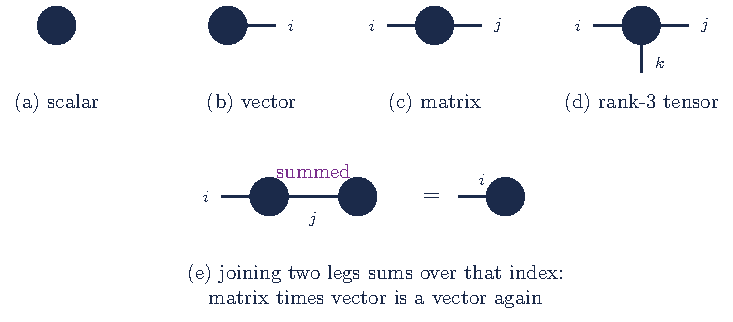
\includegraphics[width=0.80\textwidth]{figures/tensor_notation.pdf}
  \caption{Diagrammatic notation for tensors: a dot with one leg per index. (a) A scalar has no
    legs, (b) a vector has one, (c) a matrix has two, and (d) a rank-three tensor has three.
    (e) Summing over an index shared by two tensors is drawn by joining the corresponding legs
    into a single line, so a two-legged dot joined to a one-legged dot leaves one free leg and is
    therefore a vector again, exactly as matrix-vector multiplication should be.}
  \label{fig:tensor-notation}
\end{figure}

\subsection{Matrix product operators}
Hamiltonians need the same treatment. A \textbf{matrix product operator (MPO)} is the operator
version of an MPS: instead of one physical leg per site we now have two, one for the row index and
one for the column index of the local operator, plus the same two internal bond legs as before,
\begin{equation}
  \Ham = \sum_{\{\sigma_i,\sigma_i'\}} W^{\sigma_1\sigma_1'}W^{\sigma_2\sigma_2'}\cdots
    W^{\sigma_L\sigma_L'}\,\ket{\sigma_1\cdots\sigma_L}\bra{\sigma_1'\cdots\sigma_L'}.
\end{equation}
For a nearest-neighbor Hamiltonian like $\Ham_{\mathrm{Heis}} = J\sum_i \vb S_i\cdot\vb S_{i+1}$,
this internal bond dimension can be made very small, just large enough to carry ``nothing has
happened yet,'' ``an $S^x$, $S^y$, or $S^z$ was just placed and is waiting for its partner on the
next site,'' and ``the interaction has already been closed,'' so a handful of internal states per
bond is enough to represent the exact Hamiltonian, not an approximation to it.

\begin{figure}[H]
  \centering
  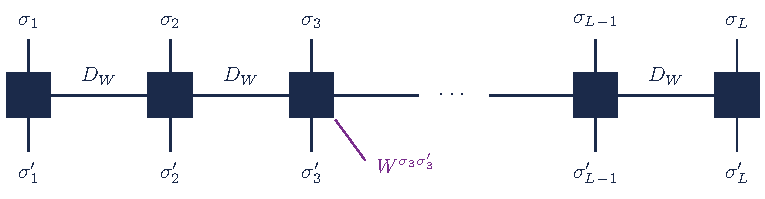
\includegraphics[width=0.85\textwidth]{figures/mpo_chain.pdf}
  \caption{A matrix product operator, the operator counterpart of the matrix product state we
    used throughout Session 4. Each site tensor $W^{\sigma_i\sigma_i'}$ carries \emph{two}
    physical legs, one for the row index $\sigma_i$ and one for the column index $\sigma_i'$, on
    top of the same two internal bond legs as before, here of dimension $D_W$. For a
    nearest-neighbor Hamiltonian those internal bonds only need to carry a handful of states,
    which is enough to encode $\Ham$ exactly rather than approximately.}
  \label{fig:mpo-chain}
\end{figure}

\subsection{Applying $\Ham$ to a state: contraction and compression}
The operation we need over and over is $\Ham\ket{\Psi}$. Diagrammatically this is simply joining the
physical legs of the MPO to the physical legs of the MPS, one site at a time, and merging the two
bond legs (one from the MPS, one from the MPO) that now run in parallel between neighboring sites
into a single, wider bond. The result is again an MPS, but with bond dimension $D\cdot D_W$, the
product of the two bond dimensions we started with. This is the practical cost of contraction: every
time we act with $\Ham$, the bond dimension grows, and if we did this repeatedly without
intervention, it would grow exponentially and defeat the whole purpose of using an MPS in the first
place. The fix is exactly the tool we already used for state compression in Session 4: a singular
value decomposition on every bond, keeping only the largest $D$ singular values (equivalently, the
$D$ largest eigenvalues of the reduced density matrix across that bond) and discarding the rest.
Because entanglement in a gapped one-dimensional system saturates at a finite value, this truncation
introduces only a small, controllable error, and is the single most important practical operation
underlying every tensor-network calculation we have run this session.

\subsection{Variational ground-state search: the DMRG sweep}
Finally, how do we actually find the ground state, rather than just apply $\Ham$ once? We treat the
MPS as a variational ansatz and minimize the energy functional directly. Introducing a Lagrange
multiplier $\lambda$ to enforce normalization, we want a stationary point of
\begin{equation}
  f[\{A\}] = \bra{\Psi[\{A\}]}\Ham\ket{\Psi[\{A\}]} - \lambda\left(\braket{\Psi[\{A\}]}-1\right).
\end{equation}
The key simplification, and the reason this is tractable at all, is that $\ket{\Psi}$ is
\emph{linear} in any single one of its tensors $A^{\sigma_i}$ once all the others are held fixed.
Setting $\partial f/\partial A^{\sigma_i} = 0$ at fixed neighbors, contracting away every tensor we
are not currently varying (on both the bra and the ket side, together with the Hamiltonian MPO)
collapses the entire, exponentially large problem down to a small effective eigenvalue equation
living only on the local physical-times-bond-times-bond space at site $i$,
\begin{equation}
  H_{\mathrm{eff}}(i)\, A^{\sigma_i} = \lambda\, A^{\sigma_i}.
\end{equation}
We diagonalize this small, dense matrix (its size is set by $D$, not by the full $2^L$-dimensional
Hilbert space), keep the lowest eigenvector as the new $A^{\sigma_i}$, then move to site $i+1$,
rebuild its effective Hamiltonian using the freshly-updated tensor at $i$, and repeat. Sweeping all
the way to the right end of the chain and back to the left, and iterating this back-and-forth sweep
until the energy stops changing, is precisely the \textbf{density matrix renormalization group
(DMRG)} algorithm: variational MPS optimization and DMRG are, in this sense, one and the same
procedure, just derived from two different historical starting points.

\begin{figure}[H]
  \centering
  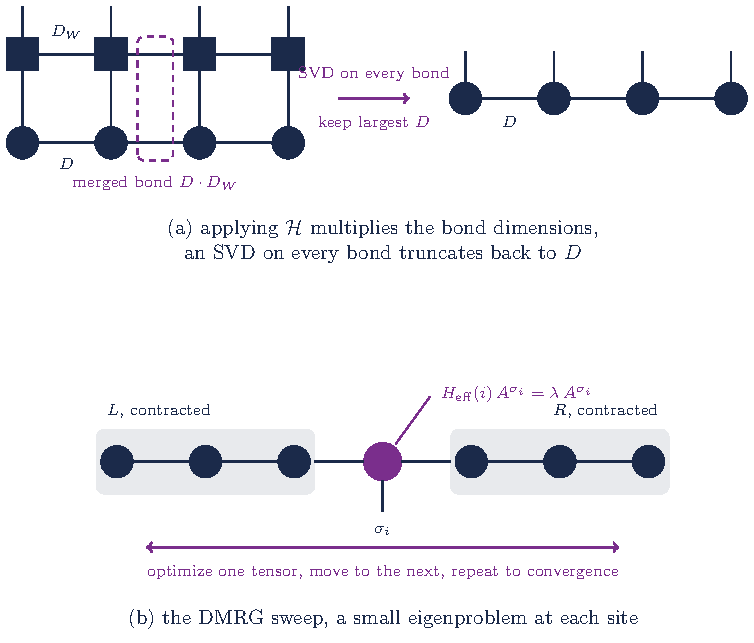
\includegraphics[width=0.78\textwidth]{figures/mps_algorithm.pdf}
  \caption{The two operations that every calculation in these two sessions is built out of.
    (a) Acting with $\Ham$, drawn by joining the matrix product operator's column legs to the
    physical legs of the state one site at a time, with the state's legs drawn pointing up here so
    that the two chains stack. The two bond legs that now run in parallel merge into a single one
    of dimension $D\cdot D_W$, so the result is again a matrix product state, just a fatter one,
    and a singular value decomposition on every bond keeping the largest $D$ values compresses it
    back. (b) The variational ground-state search. Everything except the tensor at site $i$ is
    contracted into a left and a right environment, which collapses the exponentially large problem
    to the small eigenvalue problem $H_{\mathrm{eff}}(i)A^{\sigma_i}=\lambda A^{\sigma_i}$ at that
    one site. Solving it, stepping one site over and repeating, back and forth along the chain, is
    the DMRG sweep.}
  \label{fig:mps-algorithm}
\end{figure}

\subsection{Beyond MPS: PEPS and MERA}
Matrix product states are the simplest tensor-network architecture, one tensor per site strung along
a line, and that simplicity is exactly why they are so well suited to one dimension: entanglement
across any cut of a gapped 1D chain saturates, so a finite bond dimension suffices. The natural
two-dimensional generalization, a \textbf{projected entangled pair state (PEPS)}, gives every site
one bond leg per lattice neighbor instead of just two, letting it capture the larger, area-law
entanglement of 2D systems, at the price of losing the cheap, exact contraction we relied on all
session, contracting a 2D tensor network exactly is computationally hard in general, and PEPS
calculations rely on further approximate contraction schemes. Critical, scale-invariant 1D systems
pose a related challenge even within one dimension, since their entanglement grows (logarithmically)
with subsystem size rather than saturating, which is exactly the regime the \textbf{multiscale
entanglement renormalization ansatz (MERA)} was built for, a hierarchical network of alternating
disentangling and coarse-graining tensors, layered to mirror the scale invariance of the critical
point itself. We will not develop either of these further in this course, but it is worth knowing
they exist: MPS is the first, most tractable member of a much larger family of variational tensor
architectures, each buying more entanglement capacity at the cost of a harder optimization problem.

\section*{Summary}
\begin{itemize}[nosep]
  \item The Jordan-Wigner mapping identifies the fermionic and spin-$\tfrac12$ local Hilbert spaces
    site by site, and fixes the resulting anticommutation/commutation mismatch with a string
    operator $K_i$; nearest-neighbor fermionic hopping maps onto a string-free spin term, which is
    exactly why 1D nearest-neighbor MPS methods are such a natural fit for fermionic chains.
  \item Mapping the fermionic Hamiltonian to its Jordan-Wigner spin image and solving it with MPS
    lets us redo Session 3's spinless CDW transition and Hubbard spin-charge separation at
    $L\sim100$, sharp and unambiguous, rather than blurred by the $L\lesssim16$ ceiling of exact
    diagonalization; the spinless chain's transition at $V_c\approx2t$ matches the exact XXZ result.
  \item Nonlocal particle-particle correlators distinguish gapless (power-law) from gapped
    (exponential) phases; pairing correlators, a genuinely new four-point diagnostic, show that
    repulsive interactions quench Cooper-pair fluctuations while attractive interactions enhance
    them, in both the spinless and Hubbard models.
  \item The correlation matrix built from these correlators has eigenvalues in $[0,1]$ that are
    exactly $0$ or $1$ only for a Slater determinant; the resulting correlation entropy quantifies
    how far a ground state is from any mean-field description, peaking at the spinless chain's
    phase transition and dropping smoothly as a staggered field drives the Hubbard model toward its
    mean-field, symmetry-broken solution.
  \item The general tensor-network algorithm represents states as MPS and operators as MPOs;
    applying $\Ham$ grows the bond dimension, controlled by SVD-based truncation, and the
    variational ground-state search reduces, tensor by tensor, to a sequence of small effective
    eigenvalue problems solved by sweeping back and forth along the chain, exactly the DMRG
    algorithm. PEPS and MERA extend the same idea to two dimensions and to criticality,
    respectively, beyond the scope of this course.
  \item Standing back over the whole course: mean-field theory (Session 1) gives us a cheap,
    polynomial-cost approximation that can fail qualitatively whenever the true ground state is
    genuinely entangled; exact diagonalization (Sessions 2--3) fixes that failure completely but
    only for small systems, since the Hilbert space grows exponentially; and matrix product states
    (Sessions 4--5) recover the exact many-body answer, entanglement and all, at the large,
    thermodynamically meaningful system sizes that make the underlying physics, phase transitions,
    fractionalization, spin-charge separation, unambiguous, at a cost that stays polynomial as long
    as the entanglement itself stays bounded. That progression, from product states, to unrestricted
    but tiny Hilbert spaces, to bounded-entanglement states at scale, is the single thread running
    through this entire course.
\end{itemize}

\end{document}
